\documentclass[11pt,]{article}
\usepackage{lmodern}

\usepackage{amssymb,amsmath}
\usepackage{ifxetex,ifluatex}
\usepackage{fixltx2e} % provides \textsubscript
\ifnum 0\ifxetex 1\fi\ifluatex 1\fi=0 % if pdftex
  \usepackage[T1]{fontenc}
  \usepackage[utf8]{inputenc}
\else % if luatex or xelatex
  \ifxetex
    \usepackage{mathspec}
    \usepackage{xltxtra,xunicode}
  \else
    \usepackage{fontspec}
  \fi
  \defaultfontfeatures{Mapping=tex-text,Scale=MatchLowercase}
  \newcommand{\euro}{€}
\fi
% use upquote if available, for straight quotes in verbatim environments
\IfFileExists{upquote.sty}{\usepackage{upquote}}{}
% use microtype if available
\IfFileExists{microtype.sty}{%
\usepackage{microtype}
\UseMicrotypeSet[protrusion]{basicmath} % disable protrusion for tt fonts
}{}
\usepackage[lmargin=5cm,rmargin=2.5cm,tmargin=2.5cm,bmargin=2.5cm]{geometry}

%% citation setup

\usepackage{csquotes}

\usepackage[backend=biber, maxbibnames = 99, style = apa]{biblatex}
\setlength\bibitemsep{1.5\itemsep}
\bibliography{references.bib}
\usepackage{longtable,booktabs}
\usepackage{graphicx}
\makeatletter
\def\maxwidth{\ifdim\Gin@nat@width>\linewidth\linewidth\else\Gin@nat@width\fi}
\def\maxheight{\ifdim\Gin@nat@height>\textheight\textheight\else\Gin@nat@height\fi}
\makeatother
% Scale images if necessary, so that they will not overflow the page
% margins by default, and it is still possible to overwrite the defaults
% using explicit options in \includegraphics[width, height, ...]{}
\setkeys{Gin}{width=\maxwidth,height=\maxheight,keepaspectratio}
\ifxetex
  \usepackage[setpagesize=false, % page size defined by xetex
              unicode=false, % unicode breaks when used with xetex
              xetex]{hyperref}
\else
  \usepackage[unicode=true]{hyperref}
\fi
\hypersetup{breaklinks=true,
            bookmarks=true,
            pdfauthor={Jonathan Berrisch, Timo Rammert},
            pdftitle={A Forecasting Study on Global Wine Sales},
            colorlinks=true,
            citecolor=blue,
            urlcolor=blue,
            linkcolor=magenta,
            pdfborder={0 0 0}}
\urlstyle{same}  % don't use monospace font for urls
\setlength{\parindent}{0pt}
\setlength{\parskip}{6pt plus 2pt minus 1pt}
\setlength{\emergencystretch}{3em}  % prevent overfull lines
\setcounter{secnumdepth}{5}

%%% Use protect on footnotes to avoid problems with footnotes in titles
\let\rmarkdownfootnote\footnote%
\def\footnote{\protect\rmarkdownfootnote}

%%% Change title format to be more compact
\usepackage{titling}

% Create subtitle command for use in maketitle
\newcommand{\subtitle}[1]{
  \posttitle{
    \begin{center}\large#1\end{center}
    }
}

\setlength{\droptitle}{-2em}
  \title{A Forecasting Study on Global Wine Sales}
  \pretitle{\vspace{\droptitle}\centering\huge}
  \posttitle{\par}
\subtitle{Statistical Learning}
  \author{Jonathan Berrisch, Timo Rammert}
  \preauthor{\centering\large\emph}
  \postauthor{\par}
  \predate{\centering\large\emph}
  \postdate{\par}
  \date{today}


%% linespread settings

\usepackage{setspace}

\onehalfspacing

% Language Setup

\usepackage{ifthen}
\usepackage{iflang}
\usepackage[super]{nth}
\usepackage[ngerman, english]{babel}

% Multicols for the Title page
\usepackage{multicol}

\begin{document}

\selectlanguage{english}


%\maketitle

\begin{titlepage}
  \noindent\begin{minipage}{0.6\textwidth}
	  \IfLanguageName{english}{University of Duisburg-Essen}{Universität Duisburg-Essen}\\
	  \IfLanguageName{english}{Faculty of Business Administration and Economics}{Fakultät für Wirtschaftswissensschaften}\\
	  \IfLanguageName{english}{Chair of Econometrics}{Lehrstuhl für Ökonometrie}\\
  \end{minipage}
	\begin{minipage}{0.4\textwidth}
	  \begin{flushright}
  	  \vspace{-0.5cm}
      \IfLanguageName{english}{\includegraphics*[width=5cm]{Includes/duelogo_en.png}}{\includegraphics*[width=5cm]{Includes/duelogo_de.png}}
	  \end{flushright}
	\end{minipage}
  \\
  \vspace{1.5cm}
  \begin{center}
  \huge{A Forecasting Study on Global Wine Sales}\\
  \vspace{.25cm}
  \Large{Statistical Learning}\\
  \vspace{0.5cm}
  \large{Term Paper}\\
  \vspace{1cm}
  \large{
  \IfLanguageName{english}{Submitted to the Faculty of \\ Business Administration and Economics \\at the \\University of Duisburg-Essen}{Vorgelegt der \\Fakultät für Wirtschaftswissenschaften der \\ Universität Duisburg-Essen}\\}
  \vspace{0.75cm}
  \large{\IfLanguageName{english}{from:}{von:}}\\
  \vspace{0.5cm}
  Jonathan Berrisch, Timo Rammert\\
  \end{center}
  %\vspace{2cm}
  \vfill
  \hrulefill

  \noindent\begin{minipage}[t]{0.3\textwidth}
  \IfLanguageName{english}{Reviewer:}{Erstgutachter:}
  \end{minipage}
  \begin{minipage}[t]{0.7\textwidth}
  \hspace{1cm}Prof.~Dr.~Christoph Hanck
  \end{minipage}

  \noindent\begin{minipage}[t]{0.3\textwidth}
  \IfLanguageName{english}{Deadline:}{Abgabefrist:}
  \end{minipage}
  \begin{minipage}[t]{0.7\textwidth}
  \hspace{1cm}Aug.~27th 2019
  \end{minipage}

  \hrulefill

  \begin{multicols}{3}

  Name:

  Matriculation Number:

  E-Mail:

  Study Path:

  Semester:

  Graduation (est.):

  \columnbreak

  Jonathan Berrisch

  3071485

  Jonathan@Berrisch.biz

  M.Sc. Economics

  \nth{4}

  Summer Term 2020

  \columnbreak

  Timo Rammert

  3030862

  t.rammert03@gmail.com

  M.Sc. Economics

  \nth{2}

  Winter Term 2020/2021

  \end{multicols}

\end{titlepage}


\pagenumbering{Roman}
{
\hypersetup{linkcolor=black}
\setcounter{tocdepth}{3}
\tableofcontents
}
\newpage
\listoftables
\newpage
\listoffigures
\newpage
\pagenumbering{arabic}
\hypertarget{introduction}{%
\section{Introduction}\label{introduction}}

This paper presents a forecasting study on global wine sales. This study
is based on the friberg gronqvist wine data set which is publicly
available and was previously analyzed by {[}Textcite AER Friberg,
Grönqvist{]}. Recent technological advancements led to an significant
increase in techniques that are computationally demanding and are
potentially outperforming classical statistical methods, especially in
terms of forecasting. Those techniques are usually reffered as
statistical- or machine learning methods.

We present various models which are increasingly complex. Those models
potentially gain forecasting power while losing interpretability. The
applied models range from linear regressions to tree based methods like
Random Forests and Boosting. The goal is to develop the best possible
model to forecast wine sales in litre. Although the main goal is an
accurate forecast, some of the methods used in this paper can also be
used to check whether there is an impact of expert reviews on the sales.
This effect of expert opinion on consumer demand is a quite popular
topic. E.g. {[}Textcite Hilger, Rafert, Villas Boas{]} use a field
experiment to study a review-based demand effect using wine score labels
in a retail grocery chain.

The remainder of this paper is structured as follows. Chapter 2 gives an
overview about the dataset and the preprocessing. Chapter 3 describes
the validation approach. Chapter 4 presents the models and their
specification. Chapter 5 provides the results, a conclusion and some
ideas for future research.

\hypertarget{data-and-variables}{%
\section{Data and Variables}\label{data-and-variables}}

The data set used in this paper contains 145179 observations with 59
variables. The variables include the name of the wine, the country of
origin, its price, the amount sold per week in litre, the taste segment
and variables related to different reviews among others. We need to omit
two variables beforehand, namely \enquote{time\_segm\_price} and
\enquote{artikpr}, because those are combinations of other existing
variables. Hence inclusion would lead to the problem of
multicollinearity. After omitting those two we have left the following
types of variables:

\begin{longtable}[]{@{}rrrr@{}}
\caption{Frequency of Variable Types}\tabularnewline
\toprule
Date & factor & logical & numeric\tabularnewline
\midrule
\endfirsthead
\toprule
Date & factor & logical & numeric\tabularnewline
\midrule
\endhead
1 & 8 & 19 & 29\tabularnewline
\bottomrule
\end{longtable}

Figure 1 depicts the amount of missing values in each variable. The
number of complete cases would be zero without further selection.
Therefore we exclude every variable with a ratio of missing values that
exceeds \(50\%\). In consequence 41416 observations with 45 variables
are used for building the forecasting models.

\begin{figure}
\centering
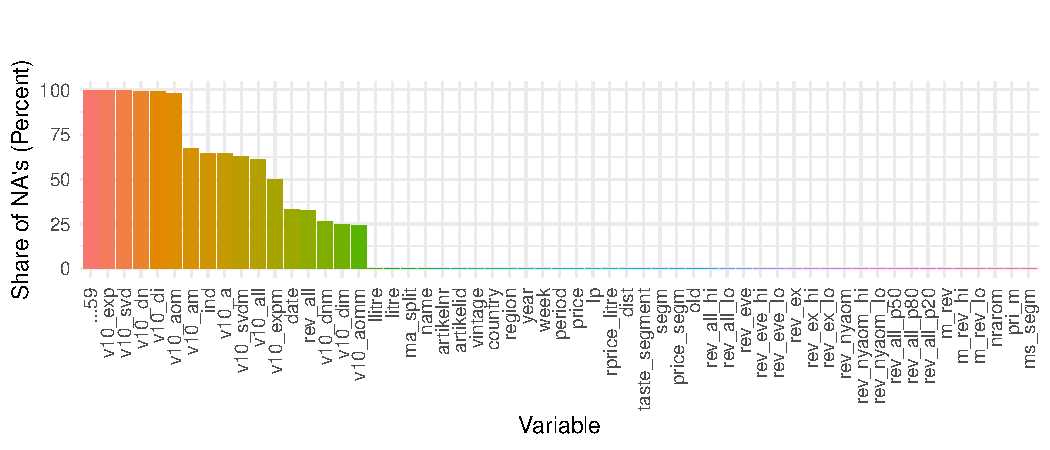
\includegraphics{../00_data/output_paper/02_missings_alt.pdf}
\caption{Share of Missing Values in the Wine Dataset}
\end{figure}

Figure XY depicts the distribution of the litre variable which is the
dependend variable in our models. One can see that the observations are
heavily skewed. The Maximum is at \(184200\) litres sold weekly while
it's minimum is near zero with only \(0.75\) litres sold per week.

\begin{figure}
\centering
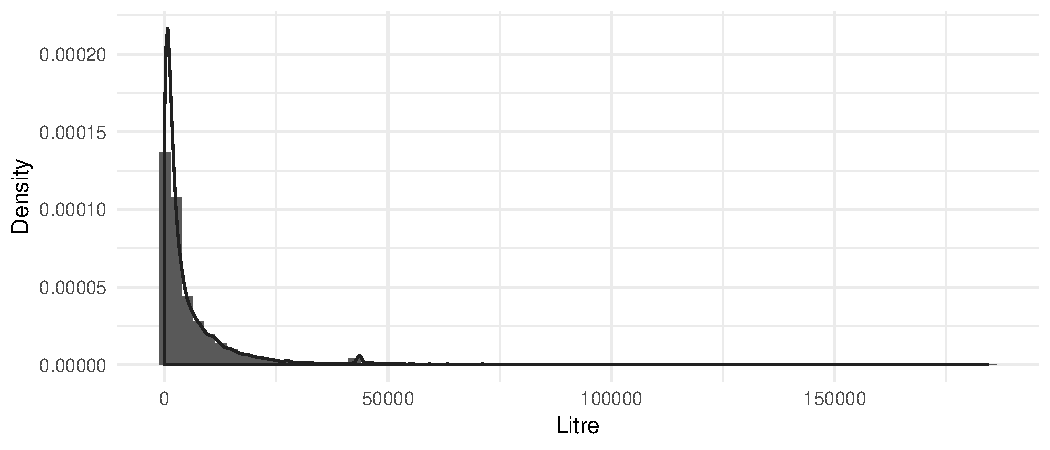
\includegraphics{../00_data/output_paper/04_hist_litre.pdf}
\caption{Histogram and Estimated Density of the Litre Variable}
\end{figure}

\hypertarget{validation-approach}{%
\section{Validation Approach}\label{validation-approach}}

Sampling may influence the model selection process because a sample
could be in favor of one specific method while another sample could lead
to different results. Therefore we validate the results of each method
using a 5-fold cross-validation. This reduces the influence of sampling
when building a training and test set while it's computationally
feasible.

In order to compute a prediction it's necessary that the test set
includes, at least all, features of the training set. Due to the high
number of levels in the countries and name variable this was not always
the case. Therefore we are using only the intersection of training and
test features to be included in the estimation.

\hypertarget{analysis}{%
\section{Analysis}\label{analysis}}

\hypertarget{mean-regression-and-linear-regression}{%
\subsection{Mean Regression and Linear
Regression}\label{mean-regression-and-linear-regression}}

At first a mean regression and a linear regression are calculated. Those
models are representing the baseline. For comparison of the different
models, the Root Mean Sqaured Error (RMSE)
\[\sqrt{\frac{1}{n}\sum_{i = 1}^{n}\left(y_i-\hat{y}_i\right)^2}\] is
calculated.

The mean regression yields an average RMSE of \(\approx 13340\) litre
sold per week. The linear regression where all variables are included
yields an average RMSE of \(\approx 5572\). The latter results is
probably influenced by overfitting. To cope with this problem we are
using variable selection and dimension reduction methods which are
discussed in the proceeding sections.

\hypertarget{lasso}{%
\subsection{Lasso}\label{lasso}}

The Least Absolute Shrinkage and Selection Operator (Lasso) is a method
combining shrinkage of the coefficent estimates to do variable
selection. It fits a linear model that is constrained by a penalty term,
i.e.~the lasso coefficients minimize:

\[
\sum_{i=1}^{n}(y_i - \beta_0 - \sum_{j=1}^{p}\beta_jx_{ij})+\lambda\sum_{j=1}^{p}|\beta_j|.
\]

Figure XY depicts the relation between lambda and the coefficients. The
crossvalidated log lambda, which minimizes the test error is
\(\approx -8.94\). At that level a total of \(\approx 666\) out of
\(713\) coefficients are
nonzero\footnote{$\approx 666.6$ to be exact, but we couldn't resists to round down.}.
The other coefficients are exactly zero due to the sparsitiy property of
the lasso estimator. Furthermore, the plot includes abbreviated variable
names of the 10 biggest coefficients. All of those coefficients are
dummys for specif*ic wine names. The average RMSE of the lasso approach
is \(\approx 5547.76\). This is a slight improvement above the linear
baseline model. The lasso slightly reduce the feature set while also
reducing the RMSE. This is evidence which supports our prior assimption
that the linear model was exposed to the problem of overfitting.
Furthermore, the coefficients of the lasso model show that the name
variable is the most important variable to explain the sold litre per
week. It is followed by the Vintage, the Region, the taste segment and
the Country of the wine. The least important variables are the review
variables which are not present in the 400 biggest coefficients.

\begin{figure}
\centering
\includegraphics{term_paper_files/figure-latex/unnamed-chunk-6-1.png}
\caption{Relation of Coefficients and Shrinkage}
\end{figure}

\hypertarget{pcr-and-pls}{%
\subsection{PCR and PLS}\label{pcr-and-pls}}

While lasso is a technique for variable selection, PCR and PLS are
methods that reduce the dimension of the feature set. Thus, the least
squares estimation is performed using a transformation of the
explanatory variables. Thereby, PLS includes the dependend variable when
computing the new feature set while PCR builds the principal components
independend of the dependend variable.

Figure XY shows the first two principal components from a principal
components analysis. The first two principal components represent
roughly 3\% of the total variance. This is a sign that the PCA doesn't
work well in our data which is might be due to the large amount of dummy
variables.

\begin{figure}
\centering
\includegraphics{term_paper_files/figure-latex/unnamed-chunk-8-1.png}
\caption{Principal Component One and Two}
\end{figure}

The results confirms the expectation. PCR has a cross validated RMSE of
\(\approx 5546.05\) while PLS leads to an RMSE of \(\approx 6201.15\).
While \(\approx 635\) principal component where included in the PCR,
only \(\approx 35.2\) components where used in the PLS. Thus PLS
significantly reduced the dimension of the featureset. While sacrificing
interpretability of the results, it leads to a higher RMSE.

\hypertarget{splines}{%
\subsection{Splines}\label{splines}}

The previous methods assumed linear relationships between the
independend variables and the dependend variable. Considering the amount
of dummy variables in the featureset the usage of nonlinear methods is
quite limited. However, to recognize potential nonlinear relationships
we add natural splines to the \(year\), \(price\), and \(rprice_litre\)
variable. Thos variables indicate the year in which the wine was
distributed, the price and the real price with Jan 2004 as base
respectively. Each natural spline was allowed to have up to 20 knots
which is sufficient to estimate complex linear relationships. The
respective RMSE's depending on the knots are presented in Figure XY.
Splines are able to improve the prediction a little which indicates that
at least some nonlinear relationship is present. However, like the
methods before, splines reduce the interpretability of the coefficients.
In this case, this tradeoff isn't offset enough by the gain in
precision. Furthermore, Figure XY shows, that the RMSE's depend to some
extend on the Fold which was used for Crossvalidation. This approves our
theoretically founded motivation to use crossvalidation.

\begin{figure}
\centering
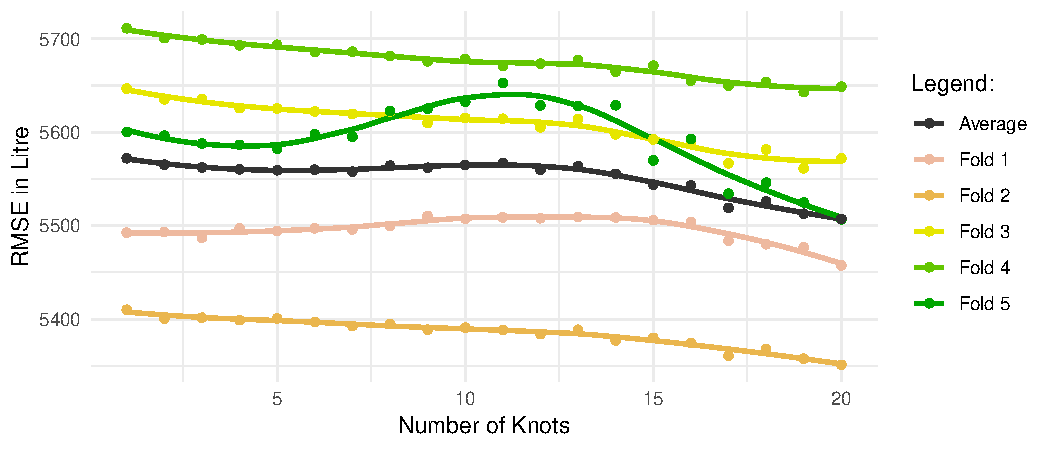
\includegraphics{../00_data/output_paper/08_splines.pdf}
\caption{Dependency Between Knots and RMSE}
\end{figure}

\hypertarget{decision-tree-methods}{%
\subsection{Decision tree methods}\label{decision-tree-methods}}

Tree-based methods utilze decision rules to split the feature space into
a number of different regions. ``Since the set of splitting rules used
to segment the predictor space can be summarized in a tree, these type
of approaches are known as decision tree methods'' {[}Textcite Hastie,
p.~303{]}. The base of tree-based methods are regression trees For
improvement of the predictive power of these methods, while losing
interpretability, one can combine different regression trees for a
single prediction. Those approaches, including bagging, random forests
and boosting, are described in more detail when being applied.

\hypertarget{regression-tree}{%
\subsubsection{Regression Tree}\label{regression-tree}}

For growing a regression tree `The algorithm needs to automatically
decide on the splitting variables and split points {[}\ldots{]} the tree
should have'\autocite[p.349]{Hastie2013}. The tree is grown when a
splitting is found that minimizes the sum of squared residuals. The
splitting is done with a greedy algorithm, i.e., at first all the data
is split into just two groups while the search of the splitting variable
and split point includes all possible variables and points
\autocite[cf.~][p.349]{Hastie2013}. After the data is split this process
is repeated for the now obtained two splitted regions until the tree is
large enough that the nodes reach a set minimum size.

\begin{figure}
\centering
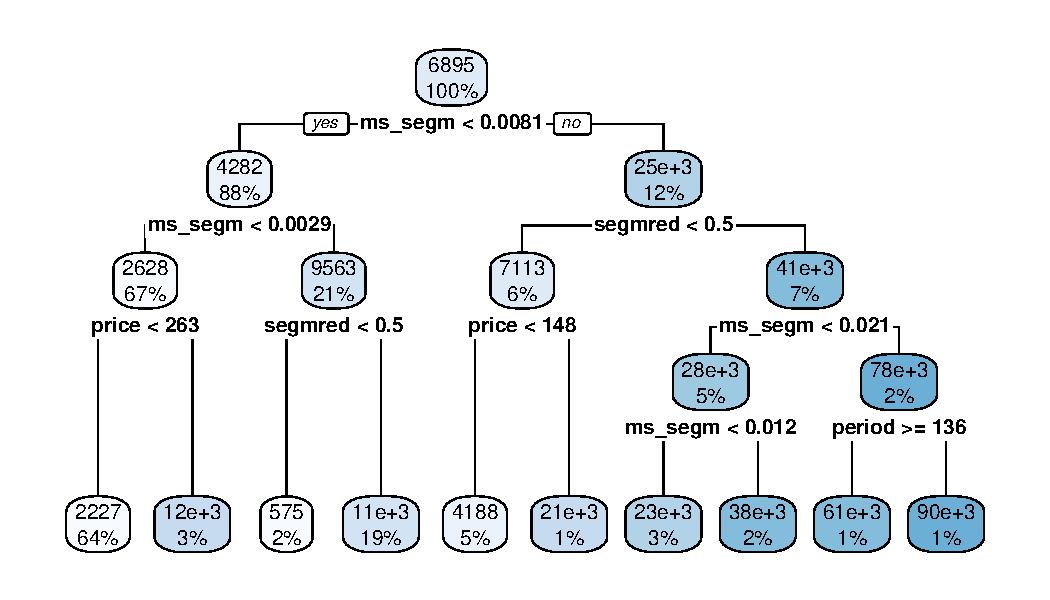
\includegraphics{../00_data/output_paper/09_tree.pdf}
\caption{Example of a Regression Tree.}
\end{figure}

Figure XY shows that only a few of the available variables are used.
These are namely \(ms_segm\), \(segmred\), \(price\), and \(period\) and
split the dataset into \(10\) parts, i.e.~the tree has got \(10\)
terminal nodes. The figure does also tell us what share of the data can
be sorted to each node, as well as the mean price of the allocated
observations. {[}{[}{[} The regression trees build in the other four
folds of the cross-validation are almost exactly the same as the shown
tree. {]}{]}{]} The selected variables indicate that according to this
method the market share, the color of the wine, the price as well as the
period. Concerning the graph and the variable \(segmred\) it is
important to keep in mind that this is a dummy variable meaning that a
value \(< 0.5\) (the left track) stands for a wine that isn't red.
Conversely the right track stands for red wines.

As regression trees may tend to grow quite large, a possible way to get
smaller trees is pruning back the grown larger tree. The goal of pruning
is `to select a subtree that leads to the lowest test error rate
{[}which{]} we can estimate {[}\ldots{]} using cross-validation or the
validation set approach' \autocite[p.~308]{James2014}. This is done by
\emph{cost complexity pruning}.

\begin{figure}
\centering
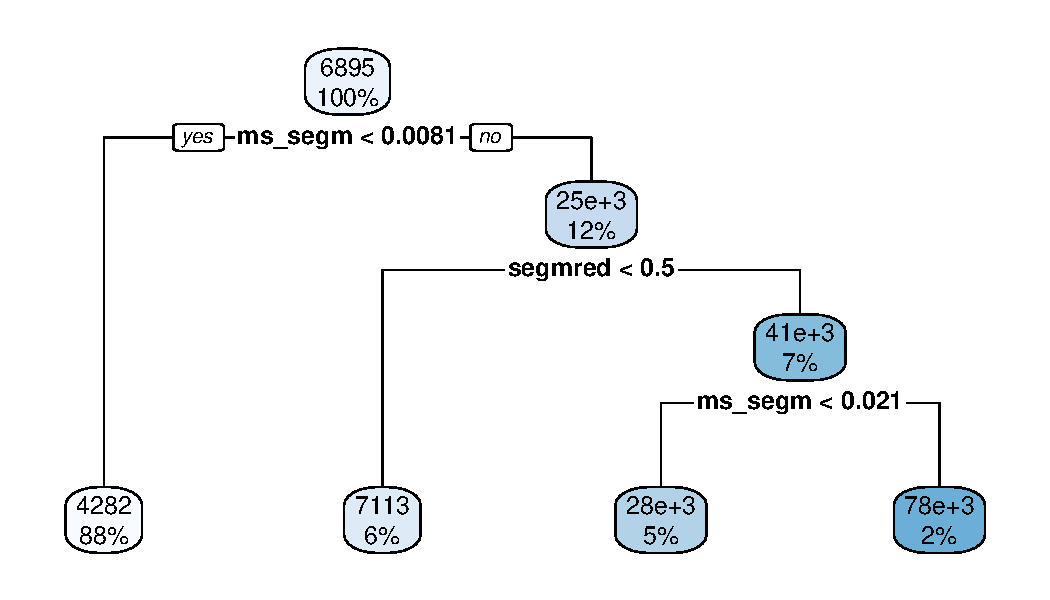
\includegraphics{../00_data/output_paper/09_tree_pruned.pdf}
\caption{Example of a Pruned Tree.}
\end{figure}

While the pruned tree might be easier to interpret, it does also come
with a higher rmse. The mean cross-validated rmse of the pruned trees is
ca. 7935.64 while the mean rmse of the normal regression trees is about
6494.75.

\hypertarget{random-forest}{%
\subsubsection{Random Forest}\label{random-forest}}

Random forests are in basic a combination of different regression trees.
The name random forest arises from the fact that at each split of the
tree a set number of randomly chosen variables are considered for the
next splitting. This results in a different tree for each iteration off
the random forest and thus by averaging leads to a lower variance than
the single trees. This is especially the case

\begin{figure}

{\centering 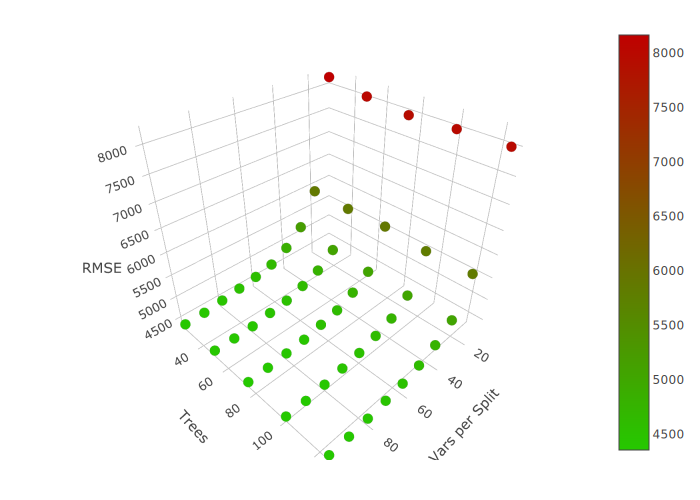
\includegraphics{../00_data/output_paper/10_rf_plot} 

}

\caption[RMSE's of the Random Forest for Different Parameters]{Dependency between RMSE, the Number of Trees and the Number of Variables Included at each Split}\label{fig:unnamed-chunk-10}
\end{figure}

\hypertarget{bagging}{%
\subsubsection{Bagging}\label{bagging}}

Bagging is a special version of a random forest in which at each split
all possible variables are taken in consideration for selection. In
contrast to random forests this may lead to very similar trees at each
iteration which thus ca be highly correlated.

\hypertarget{boosting}{%
\subsubsection{Boosting}\label{boosting}}

\begin{figure}

{\centering 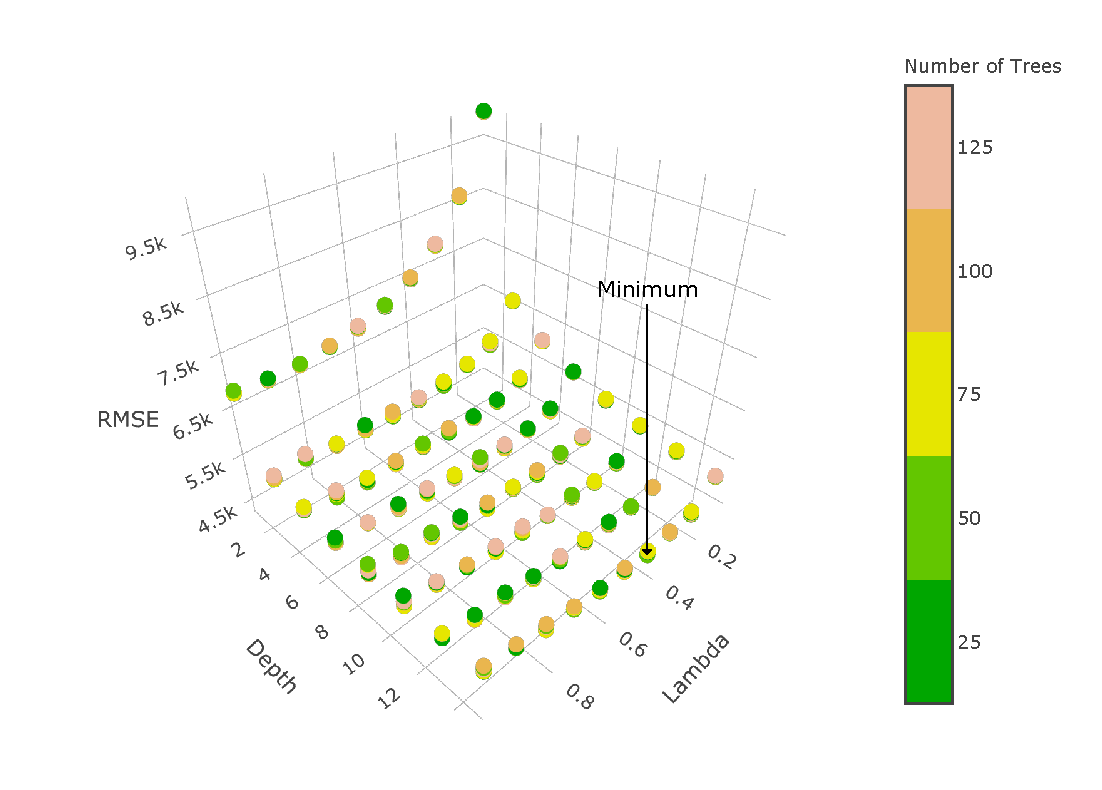
\includegraphics{../00_data/output_paper/11_boosting_plot} 

}

\caption[RMSE's of the Boosting Model for Different Parameters]{Dependency between RMSE, Lambda, the Depths and the Number of Trees that are Grown}\label{fig:unnamed-chunk-11}
\end{figure}

In contrast to random forests boosting grows tree sequentially meaning
that for every new tree information from already grown trees is used
\autocite[p.322]{James2014}. For boosting rather small regression trees
are used to improve the boosting tree slowly. This is achieved by taking
the residuals from the current boosting tree, fitting a (small) tree to
these residuals and then fiiting this tree into the boosting tree in
areas where the performance of the boosting tree could be improved
\autocite[p.322]{James2014}.

\hypertarget{conclusion}{%
\section{Conclusion}\label{conclusion}}

\pagebreak

\hypertarget{citations}{%
\subsection{Citations}\label{citations}}

\pagebreak

\hypertarget{annotations}{%
\subsection{Annotations}\label{annotations}}

\hypertarget{overview-over-the-rmses}{%
\subsubsection{Overview over the RMSEs}\label{overview-over-the-rmses}}

\begin{tabular}{l|r|r}
\hline
Method & RMSE & No..of.Variables\\
\hline
Mean-Regression & 0 & 0\\
\hline
Linear Regression & 0 & 0\\
\hline
Forword Stepwise Selection & 0 & 0\\
\hline
Backward Stepwise Selection & 0 & 0\\
\hline
Regression Tree & 0 & 0\\
\hline
Pruned Tree & 0 & 0\\
\hline
Random Forest & 0 & 0\\
\hline
\end{tabular}
\renewcommand*{\mkbibnamefamily}[1]{\textbf{#1}}
\renewcommand*{\mkbibnamegiven}[1]{\textbf{#1}}
\renewcommand*{\mkbibnameprefix}[1]{\textbf{#1}}
\renewcommand*{\mkbibnamesuffix}[1]{\textbf{#1}}
\printbibliography[title=References]

\newpage
\textbf{Eidesstattliche Versicherung}

\bigskip

Ich versichere an Eides statt durch meine Unterschrift, dass ich die vorstehende Arbeit selbständig und ohne fremde Hilfe angefertigt und alle Stellen, die ich wörtlich oder annähernd wörtlich aus Veröffentlichungen entnommen habe, als solche kenntlich gemacht habe, mich auch keiner anderen als der angegebenen Literatur oder sonstiger Hilfsmittel bedient habe. Die Arbeit hat in dieser oder ähnlicher Form noch keiner anderen Prüfungsbehörde vorgelegen.

\vspace{1cm}
\rule{0pt}{2\baselineskip} %
\par\noindent\makebox[2.25in]{\indent Essen, den \hrulefill} \hfill\makebox[2.25in]{\hrulefill}%
\par\noindent\makebox[2.25in][l]{} \hfill\makebox[2.25in][c]{Jonathan Berrisch, Timo Rammert}%


\end{document}
